% Digital Logic Report Template
% Created: 2020-01-10, John Miller

%==========================================================
%=========== Document Setup  ==============================

% Formatting defined by class file
\documentclass[11pt]{article}

% ---- Document formatting ----
\usepackage[margin=1in]{geometry}	% Narrower margins
\usepackage{booktabs}				% Nice formatting of tables
\usepackage{graphicx}				% Ability to include graphics

%\setlength\parindent{0pt}	% Do not indent first line of paragraphs 
\usepackage[parfill]{parskip}		% Line space b/w paragraphs
%	parfill option prevents last line of pgrph from being fully justified

% Parskip package adds too much space around titles, fix with this
\RequirePackage{titlesec}
\titlespacing\section{0pt}{8pt plus 4pt minus 2pt}{3pt plus 2pt minus 2pt}
\titlespacing\subsection{0pt}{4pt plus 4pt minus 2pt}{-2pt plus 2pt minus 2pt}
\titlespacing\subsubsection{0pt}{2pt plus 4pt minus 2pt}{-6pt plus 2pt minus 2pt}

% ---- Hyperlinks ----
\usepackage[colorlinks=true,urlcolor=blue]{hyperref}	% For URL's. Automatically links internal references.

% ---- Code listings ----
\usepackage{listings} 					% Nice code layout and inclusion
\usepackage[usenames,dvipsnames]{xcolor}	% Colors (needs to be defined before using colors)

% Define custom colors for listings
\definecolor{listinggray}{gray}{0.98}		% Listings background color
\definecolor{rulegray}{gray}{0.7}			% Listings rule/frame color

% Style for Verilog
\lstdefinestyle{Verilog}{
	language=Verilog,					% Verilog
	backgroundcolor=\color{listinggray},	% light gray background
	rulecolor=\color{blue}, 			% blue frame lines
	frame=tb,							% lines above & below
	linewidth=\columnwidth, 			% set line width
	basicstyle=\small\ttfamily,	% basic font style that is used for the code	
	breaklines=true, 					% allow breaking across columns/pages
	tabsize=3,							% set tab size
	commentstyle=\color{gray},	% comments in italic 
	stringstyle=\upshape,				% strings are printed in normal font
	showspaces=false,					% don't underscore spaces
}

% How to use: \Verilog[listing_options]{file}
\newcommand{\Verilog}[2][]{%
	\lstinputlisting[style=Verilog,#1]{#2}
}




%======================================================
%=========== Body  ====================================
\begin{document}

\title{ELC 2137 Lab \#\#: Lab Title}
\author{Put your name(s) here}

\maketitle


\section*{Summary}

In this lab, we built a conditional adder, 6, and 11-bit binary to BCD converter using the dibble dabble algorithm. We used the same seven-segment display decoder to implement the code to hardware.


\section*{Code}

\Verilog[firstline=23, caption=Add3 ,label=code:file_1]{add3.sv}
\Verilog[firstline=23, caption=Add3 Test ,label=code:file_2]{add3_test.sv}
\Verilog[firstline=23, caption=6 bit BCD,label=code:file_3]{BCD6b.sv}
\Verilog[firstline=23, caption=Sseg 6 bit BCD Test ,label=code:file_4]{BCD6b_test.sv}
\Verilog[firstline=23, caption=11 bit BCD ,label=code:file_5]{BCD11b.sv}
\Verilog[firstline=23, caption=11 bit BCD Test ,label=code:file_6]{BCD11b_test.sv}
\Verilog[firstline=23, caption=Sseg1 for BCD,label=code:file_7]{sseg1_BCD.sv}

\section*{Results}

\begin{figure}[ht]\centering
	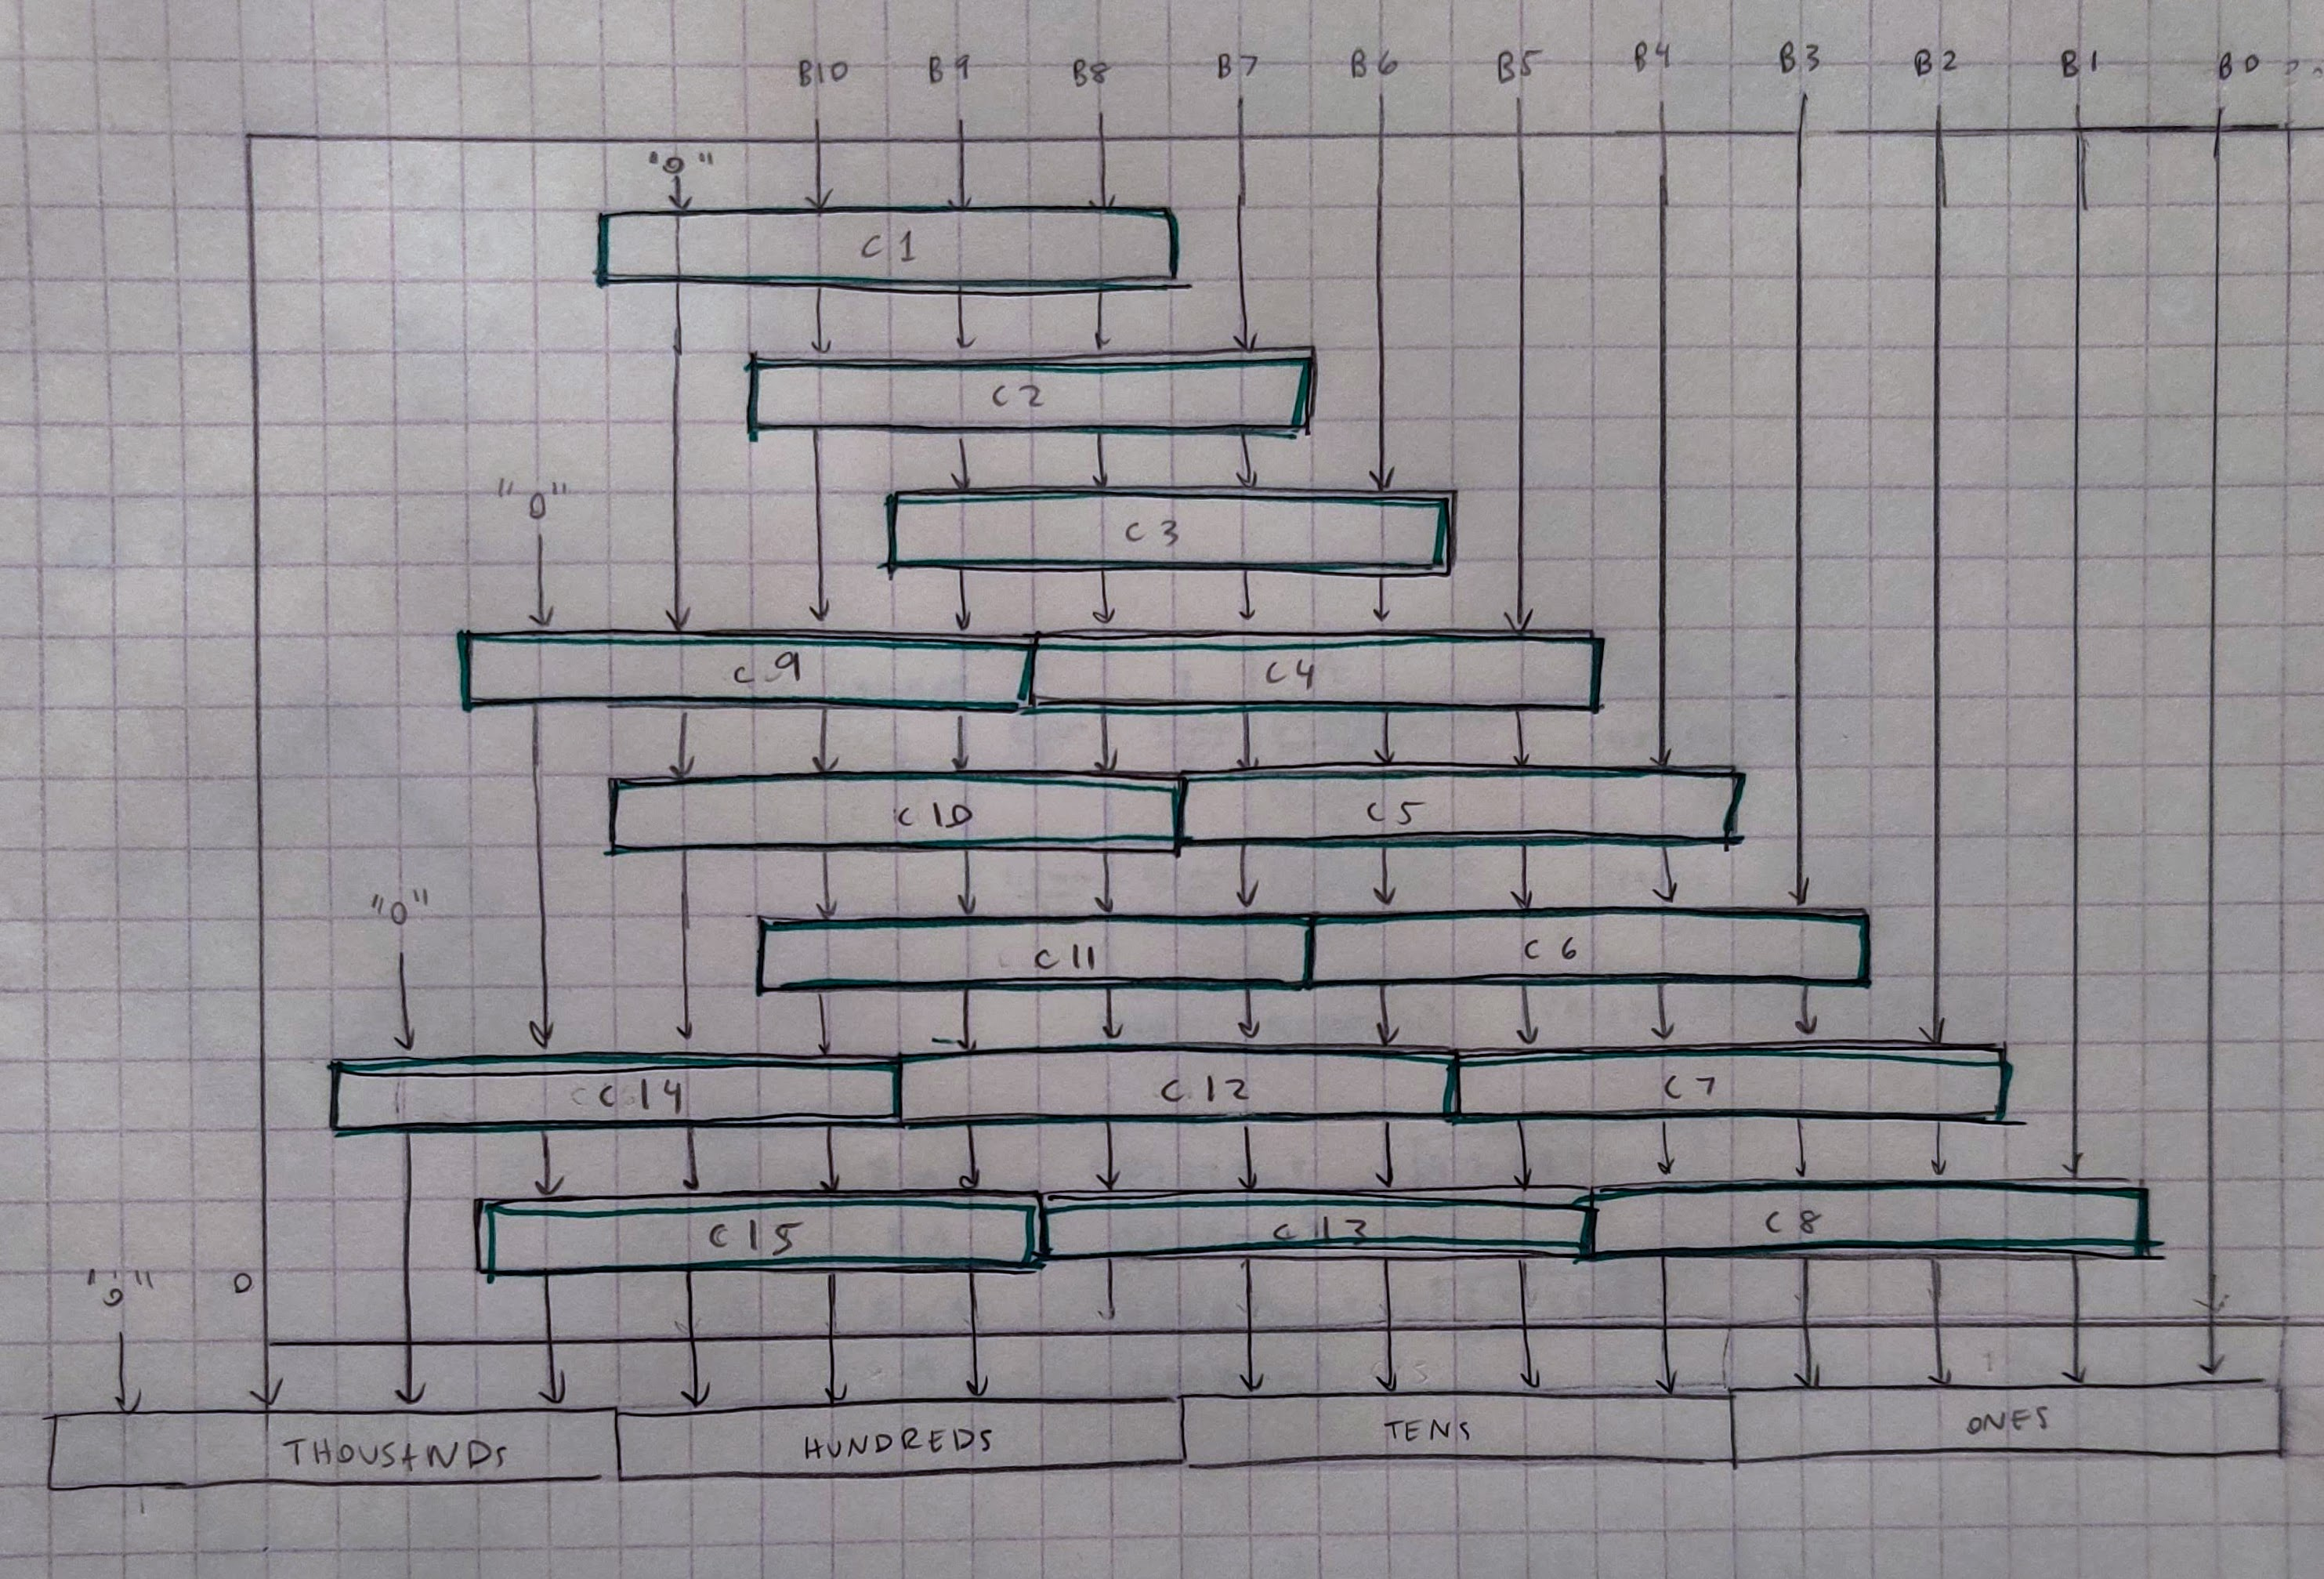
\includegraphics[width=.75\textwidth]{ckt_diagram_11b}
	\caption{Circuit Diagram for 11 bit converter}
	\label{fig:b3_0}			
\end{figure}

\begin{figure}[ht] \centering
	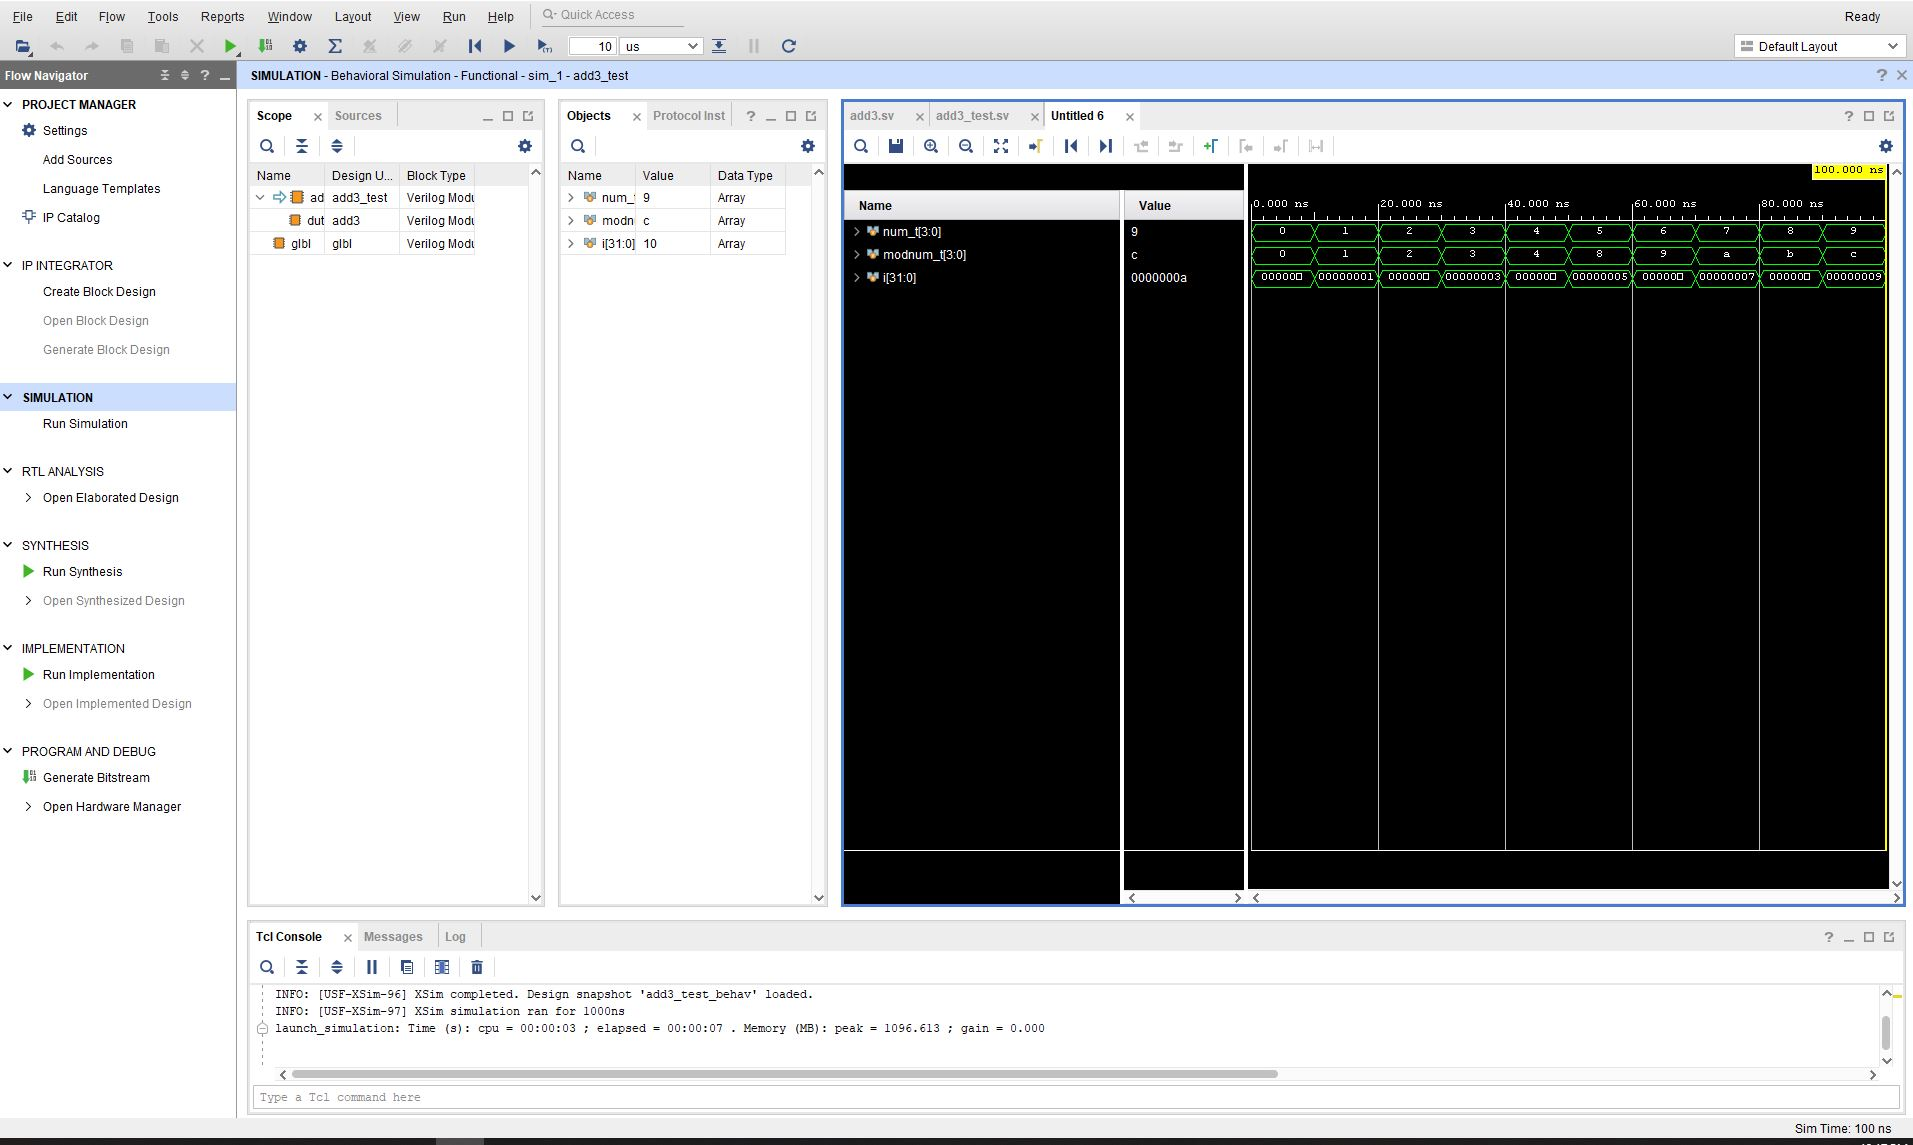
\includegraphics[width=1\textwidth,trim=32cm 20cm 0cm 4cm,clip]{add3_test_screen}
	\caption{Add 3}
	\label{fig:img1}
\end{figure}


\begin{figure}[ht] \centering
	
	\begin{tabular}{c|cc}
		\toprule
		B & tens & ones \\
		\midrule
		000000 & 0000 & 0000 \\
		000001 & 0000 & 0001 \\
		000010 & 0000 & 0010 \\
		000011 & 0000 & 0011 \\
		000100 & 0000 & 0100 \\
		\bottomrule
	\end{tabular}
 
	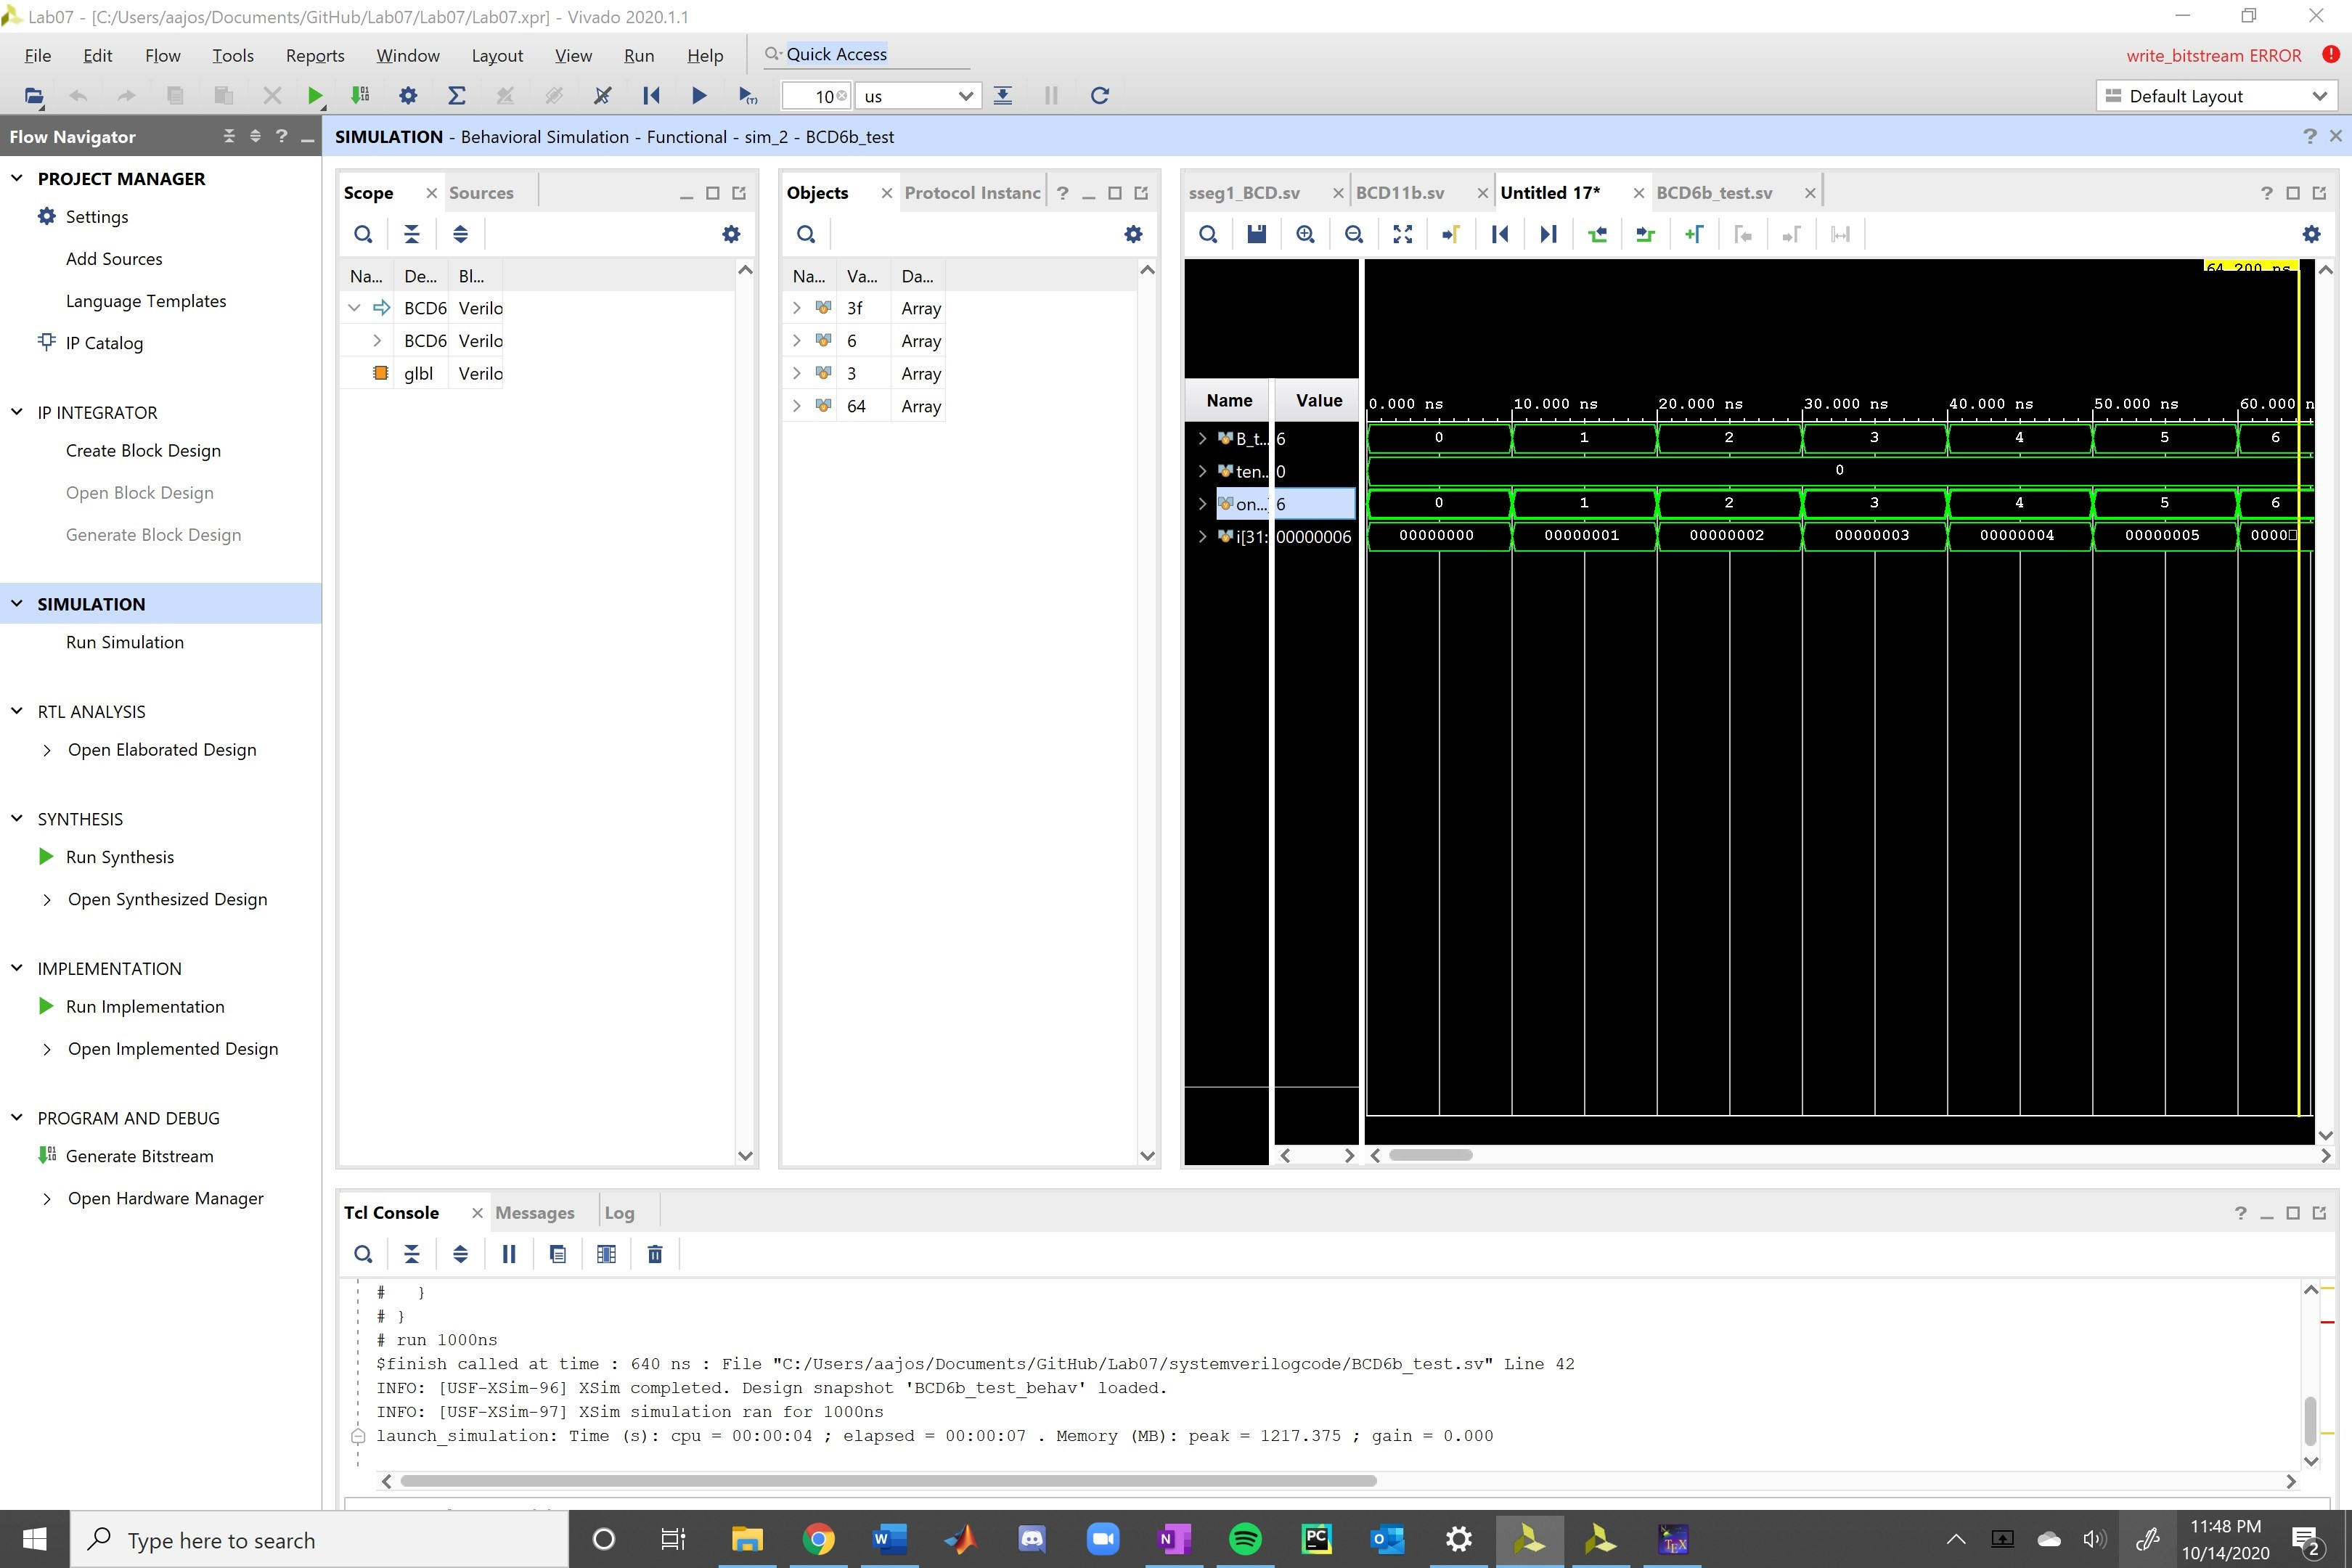
\includegraphics[width=1\textwidth,trim=19cm 15cm 0cm 6cm,clip]{BCD6b_test_screen}
	\caption{6 bit BCD beginning}
	\label{fig:img2}
\end{figure}

 

\begin{figure}[ht] \centering
	
	\begin{tabular}{c|cc}
		\toprule
		B & tens & ones \\
		\midrule
		111011 & 0101 & 1001 \\
		111100 & 0110 & 0000 \\
		111101 & 0110 & 0001 \\
		111110 & 0110 & 0010 \\
		111111 & 0110 & 0011 \\
		\bottomrule
	\end{tabular}
	
	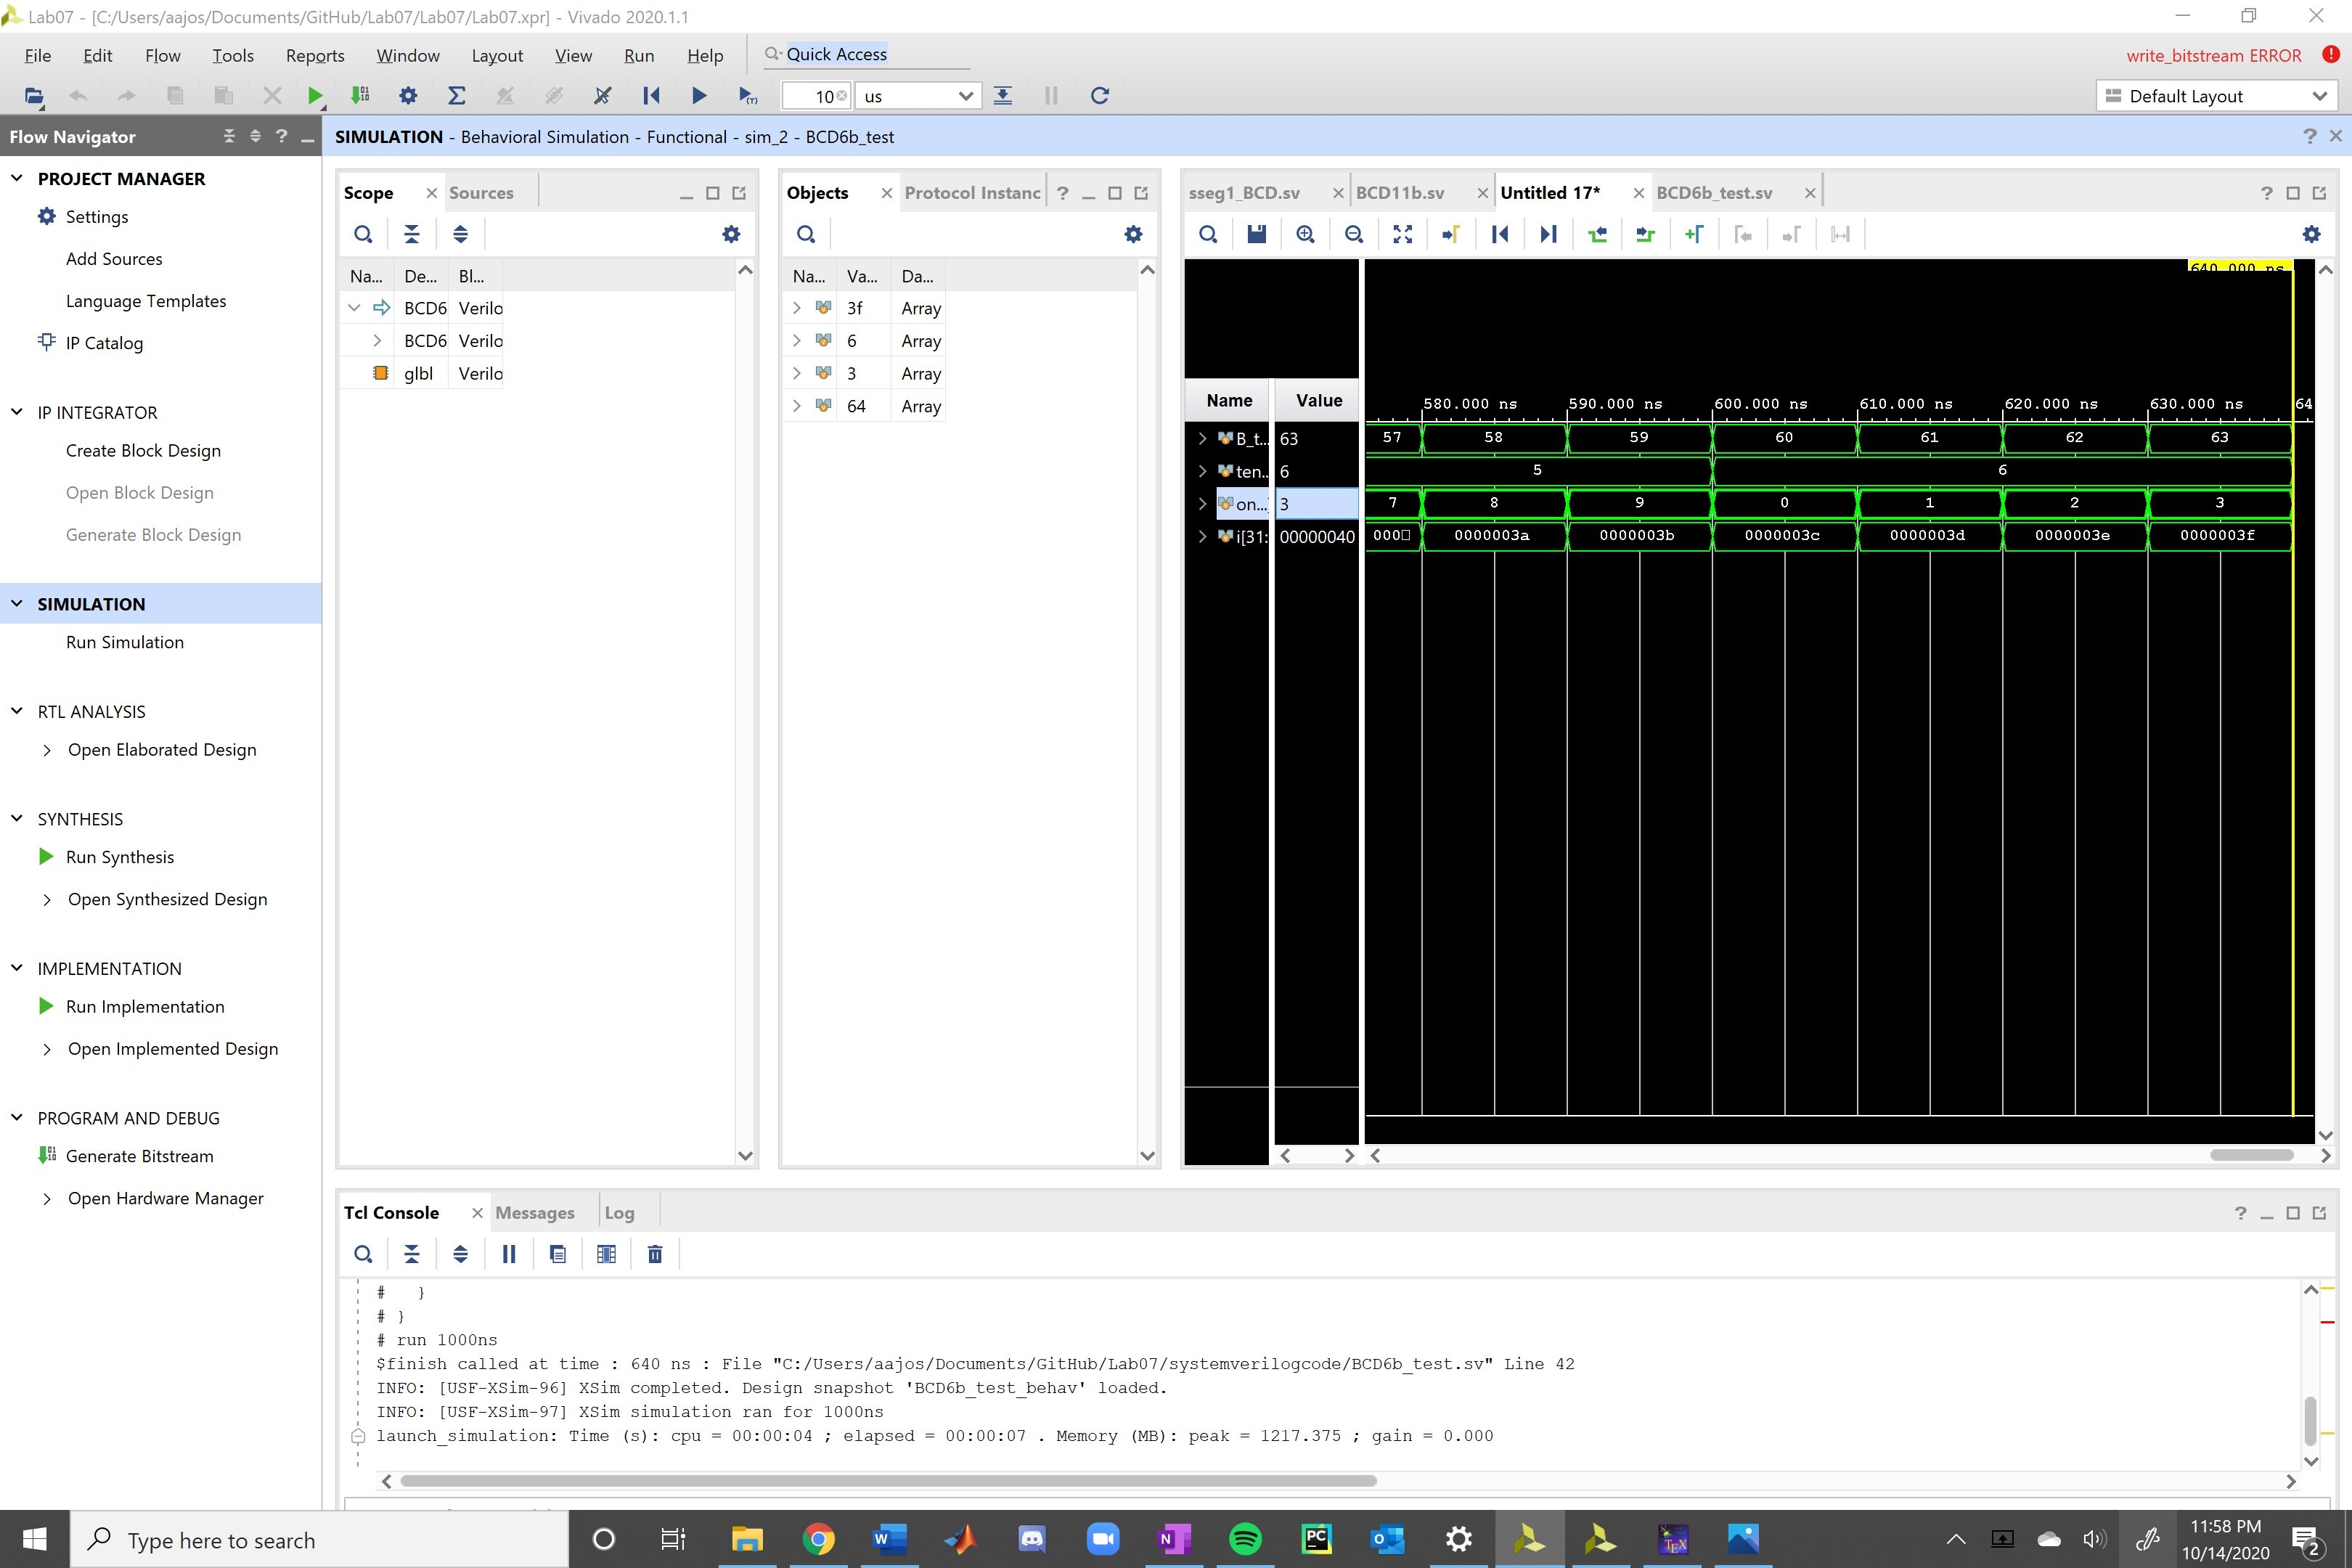
\includegraphics[width=1\textwidth,trim=19cm 14cm 0cm 6cm,clip]{BCD6b_test_screen1}
	\caption{6 bit BCD end} 
	\label{fig:img3}
\end{figure}
 

\begin{figure}[ht] \centering
	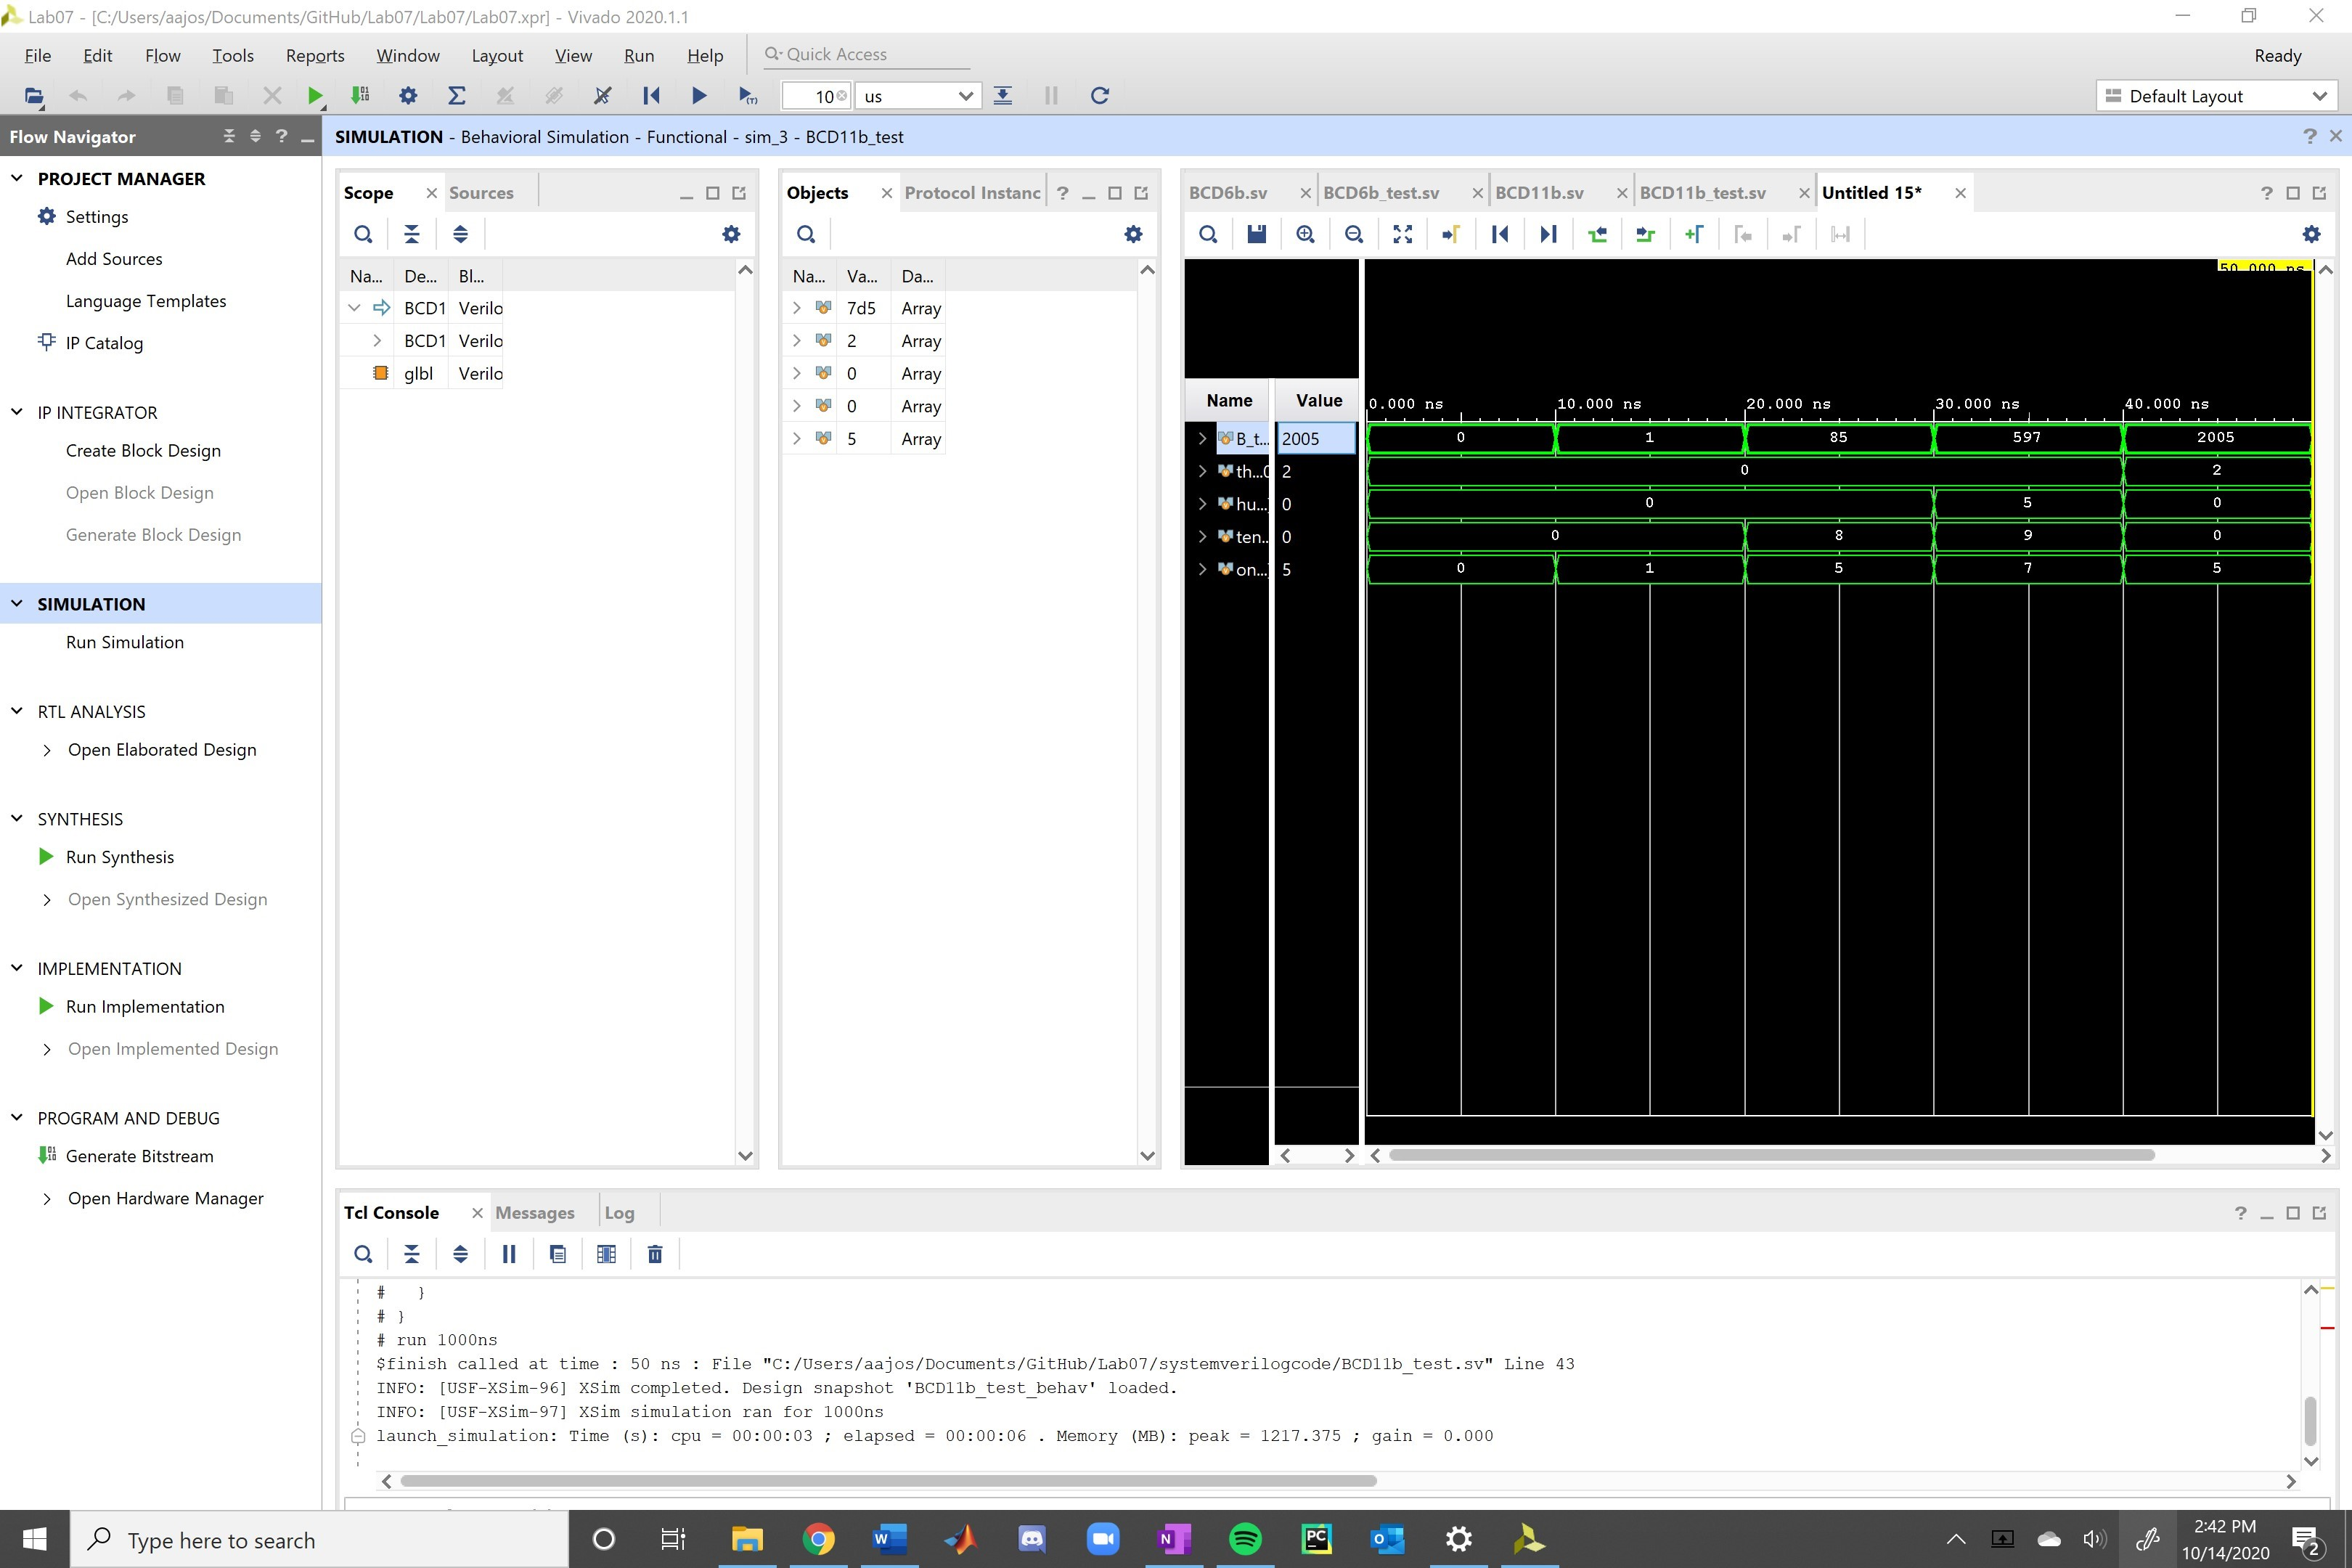
\includegraphics[width=1\textwidth,trim=19cm 14cm 0cm 6cm,clip]{BCD11b_test_screen}
	\caption{11 bit BCD test cases}
	\label{fig:img4}
\end{figure}

\end{document}
